%! Author = joels
%! Date = 05/01/2021

\section{Architektur und fortgeschrittene Themen}
\subsection{Schichtenarchitektur}
Wichtig ist, dass keine zyklischen Abhängigkeiten entstehen. Domain sollte zum Beispiel nie von View abhängen.\\
Beispiele für Möglichkeiten zur Entkopplung an Grenzen:\\
\textcolor{blue}{Observer Pattern, Interfaces und Dependency Injection}\\
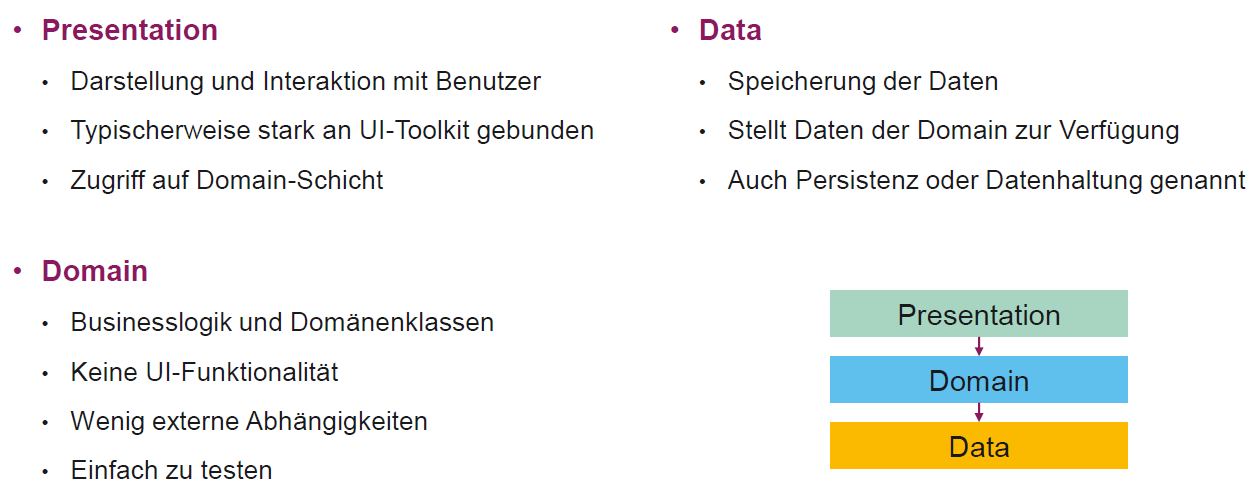
\includegraphics{schichtenarchitektur.png}
\subsection{Observer Pattern}
\textbf{Zwei Rollen:}\\
\textcolor{blue}{Sobject:} Wird beobachtet, z.B. Model-Klasse\\
\textcolor{blue}{Observer:} Beobachter, z.B. View-Klasse\\
$\rightarrow$ Observer registrieren sich beim Subject für Statusänderungen.\\
$\rightarrow$ Observer Pattern wird oft mit MVC kombiniert
\subsection{Model-View-Controller}
\begin{minipage}{0.65\linewidth}
    \textbf{Pattern für die Organisation der Presentation:}\\
    \textcolor{blue}{Model} beinhaltet die Daten. (Java-Klassen)\\
    \textcolor{blue}{View} liest die Daten des Modells und zeigt diese an. (View, Adapter)\\
    \textcolor{blue}{Controller} erhält Events der View und manipuliert das Model. (Activity, Fragment)\\
    Kritik: Viel Code im Controller.
\end{minipage}
\begin{minipage}{0.3\linewidth}
    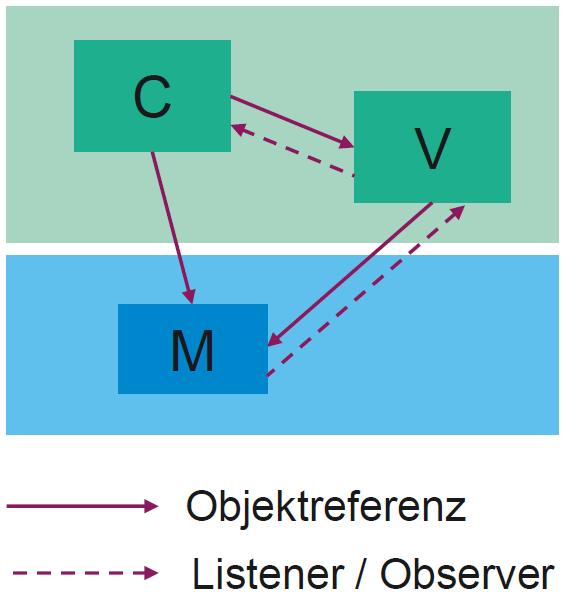
\includegraphics{mvc.png}
\end{minipage}
\subsection{Application Methoden}
\textbf{\textcolor{blue}{onCreate()}}: Einmalig nach dem Start der App. Vor Erzeugung anderer App-Komponenten\\
\textbf{\textcolor{blue}{onTerminate()}}: Wird auf realen Geräten nie aufgerufen. Reminder: Apps können stets beendet werden\\
\textbf{\textcolor{blue}{onConfigurationChanged(newConfig)}}: Bei Änderungen der System-Konfiguration. Parameter enthält neue Konfiguration. Beispiel: Rotation des Gerätes\\
\textbf{\textcolor{blue}{onLowMemory()}}: Bei Speicherknappheit des Systems. Hinweis auf mögliche Terminierung der App\\
\textbf{\textcolor{blue}{onTrimMemory(level)}}: Bei geeigneten Momenten für Aufräumaktionen. Parameter gibt Hinweise auf Auslöser. Beispiel: App geht in den Hintergrund (TRIM\_MEMORY\_UI\_HIDDEN)\\
$\rightarrow$ Via \textcolor{blue}{Application-Klasse} kann der Lebenszyklus aller Activities überwacht werden. Implementierung und Registrierung von \textcolor{blue}{Application.ActivityLifeCycleCallbacks}
\subsection{Context}
Context ist eine abstrakte Klasse der SDK mit über 50 Ableitungen, beispielsweise Activity und Application. Sie erlaubt den Zugriff auf Dienste und Ressourcen der App. z.B:
\begin{itemize}[topsep=0pt, leftmargin=4mm]
    \setlength\itemsep{-0.3em}
    \item Context.startActivity()
    \item new Intent(Context, Type)
    \item LayoutInflater.from(Context)
    \item Toast.makeText(Context, String, int)
    \item NotificationManagerCompat.from(Context)
\end{itemize}
\subsection{Broadcasts}
\begin{itemize}[topsep=0pt, leftmargin=4mm]
    \setlength\itemsep{-0.3em}
    \item Für den Austausch von meldungen zwischen Apps. (Publish-Subscribe-Pattern)
    \item Zwei Arten von Broadcasts: \textcolor{blue}{Lokal}: innerhalb der App. \textcolor{blue}{Global:} Innerhalb des ganzen Systems.
    \item Android sendet selbst globale Broadcasts (System gestartet, Netzwerkverbindung verloren, SMS empfangen, etc.)
\end{itemize}
\subsubsection{Broadcasts empfangen}
Dynamische Registrierung via Context: An Lebenszeit des Contexts gebunden. Abmelden von Events nicht vergessen.
\begin{lstlisting}
// MyReceiver.java
public class MyBroadcastReceiver extends BroadcastReceiver {
    @Override
    public void onReceive(Context context, Intent intent) {
        Log.d(null, "Broadcast: " + intent.getAction());
    }
}

// AndroidManifest.xml
<application>
    <receiver android:name=".MyBroadcastReceiver">
        <intent-filter>
            <action android:name="android.intent.action.TIME_SET"/>
        </intent-filter>
    </receiver>
</application>

// MainActivity.java
// Registrierung
BroadcastReceiver receiver = new MyBroadcastReceiver();
String action = ConnectivityManager.CONNECTIVITY_ACTION;
IntentFilter filter = new IntentFilter(action);
registerReceiver(receiver, filter);
// Abmeldung
unregisterReceiver(receiver);
\end{lstlisting}
\subsubsection{Broadcasts versenden}
Broadcasts sind normale Intent-Objekte. Die Action im Intent definiert den Ereignistyp. Parameter sind als Extras möglich.
\begin{lstlisting}
// AndroidManifest.xml
<application>
    <receiver android:name=".MyBroadcastReceiver">
        <intent-filter>
            <action android:name="ch.ost.rj.mge.v06.MY_INTENT" />
        </intent-filter>
    </receiver>
</application>

// MainActivity.java
// Registrierung
BroadcastReceiver receiver = new MyBroadcastReceiver();
String action = "ch.ost.rj.mge.v06.MY_INTENT";
IntentFilter filter = new IntentFilter(action);
registerReceiver(receiver, filter);

// Impliziter Broadcast
Intent intent = new Intent();
intent.setAction(action);
sendBroadcast(intent);

// Expliziter Broadcast
Intent intent = new Intent(this, MyBroadcastReceiver.class);
intent.setAction(action);
sendBroadcast(intent);
\end{lstlisting}
\subsubsection{Best Practices}
\begin{itemize}[topsep=0pt, leftmargin=4mm]
    \setlength\itemsep{-0.3em}
    \item Dynamische Registrierung bevorzugen
    \item Lokale Broadcasts bevorzugen
    \item Keine sensitiven Daten in Broadcasts übermitteln
    \item App ID in eigene Broadcast-Actions integrieren
    \item Schnelle Rückkehr aus onReceive()
\end{itemize}

\subsection{Services}
\begin{itemize}[topsep=0pt, leftmargin=4mm]
    \setlength\itemsep{-0.3em}
    \item Für die Ausführung von Aktionen im Hintergrund
    \begin{itemize}[topsep=0pt, leftmargin=4mm]
        \setlength\itemsep{-0.3em}
        \item Laden von Daten über Netzwerk
        \item Streaming von Musik
        \item Rechenintensive Aufgaben
    \end{itemize}
    \item Lebenszyklus unabhängig von App
    \item Kein oder reduziertes UI (Notification)
    \item Werden auf Main-Thread ausgeführt
    \begin{itemize}[topsep=0pt, leftmargin=4mm]
        \setlength\itemsep{-0.3em}
        \item Service: Aufgabe von Activity entkoppeln
        \item Thread: Aufgabe von Main-Thread entkoppeln
    \end{itemize}
\end{itemize}
\subsubsection{Started Services}
\begin{itemize}[topsep=0pt, leftmargin=4mm]
    \setlength\itemsep{-0.3em}
    \item Für einmalige Aktionen
    \item Laufen potentiell endlos weiter
    \begin{itemize}[topsep=0pt, leftmargin=4mm]
        \setlength\itemsep{-0.3em}
        \item Beendigung durch Service selbst: stopSelf()
        \item Beendigung durch eine Applikation: stopService()
        \item Beendigung durch Android
    \end{itemize}
    \item Spezialvarianten
    \begin{itemize}[topsep=0pt, leftmargin=4mm]
        \setlength\itemsep{-0.3em}
        \item IntentService für Ausführung in Background-Thread und automatischem Stopp
        \item JobIntentService als modernere Alternative für IntentService
        \item Foreground Services mit Notifications als UI
    \end{itemize}
\end{itemize}
\subsubsection{Bound Services}
\begin{itemize}[topsep=0pt, leftmargin=4mm]
    \setlength\itemsep{-0.3em}
    \item Für Aufgaben über längere Zeitdauer
    \item Client-Server ähnliche Kommunikation
    \begin{itemize}[topsep=0pt, leftmargin=4mm]
        \setlength\itemsep{-0.3em}
        \item Innerhalb eines Apps: via Interface
        \item App-übergreifend: via Messenger-Klasse
    \end{itemize}
    \item Austausch von Daten fester Bestandteil
    \item Mehrere Clients gleichzeitig möglich
    \item Nach Verbindungsende zu letztem Client wird der Service automatisch gestoppt
\end{itemize}

\subsection{Build \& Deployment}
Apps werden aus APK-Dateien installiert. APKs aus dem Play Store sind signiert.\\
\textbf{\textcolor{blue}{APK Splitting/Expansion Files:}}\\
\begin{itemize}[topsep=0pt, leftmargin=4mm]
    \setlength\itemsep{-0.3em}
    \item Limit des Google Play Store: 100 MB
    \begin{itemize}[topsep=0pt, leftmargin=4mm]
        \setlength\itemsep{-0.3em}
        \item Keine technische Grenze des APK-Formats
        \item Schutz der Infrastruktur und User
    \end{itemize}
    \item Optimierung 1: APK Splitting
    \begin{itemize}[topsep=0pt, leftmargin=4mm]
        \setlength\itemsep{-0.3em}
        \item Aufteilung in verschiedene kleinere APKs
        \item Kriterien: CPU-Architektur, Gerätetyp, ...
    \end{itemize}
    \item Optimierung 2: APK Expansion Files
    \begin{itemize}[topsep=0pt, leftmargin=4mm]
        \setlength\itemsep{-0.3em}
        \item Für speicherintensive Ressourcen (z.B. Videos)
        \item Play Store erlaubt max. 2 x 2 GB zusätzlich
        \item ZIP-Archive mit Dateiendung .OBB
    \end{itemize}
\end{itemize}
\textbf{\textcolor{blue}{ABB (Android App Bundle):}}\\
\begin{itemize}[topsep=0pt, leftmargin=4mm]
    \setlength\itemsep{-0.3em}
    \item Nachfolger des APK-Formats
    \item Container mit jeglichen Inhalten eines Apps
    \item Dynamische Erzeugung von APKs
    \begin{itemize}[topsep=0pt, leftmargin=4mm]
        \setlength\itemsep{-0.3em}
        \item Optimierte Dateigrösse
        \item Play Feature Delivery für Feature-Module
        \item Play Asset Delivery als Nachfolger von OBB
    \end{itemize}
    \item Konsequenzen
    \begin{itemize}[topsep=0pt, leftmargin=4mm]
        \setlength\itemsep{-0.3em}
        \item Google in Besitz des Signaturschlüssels
        \item Neues Limit von 150 MB für ABB-Datei
    \end{itemize}
    \item Ab 2021 zwingend im Google Play Store
\end{itemize}